\subsection{PMOS threshold}\label{pmos_dimensioning}
Now we take a look at the worst case of 4 stacked PMOS transistors, which is the highest stacking amount which will be possible in technologies relying on this process.
%%  ************    LibreSilicon's StdCellLibrary   *******************
%%
%%  Organisation:   Chipforge
%%                  Germany / European Union
%%
%%  Profile:        Chipforge focus on fine System-on-Chip Cores in
%%                  Verilog HDL Code which are easy understandable and
%%                  adjustable. For further information see
%%                          www.chipforge.org
%%                  there are projects from small cores up to PCBs, too.
%%
%%  File:           StdCellLib/Documents/LaTeX/schematic_OR4.tex
%%
%%  Purpose:        Schematic File for OR4
%%
%%  ************    LaTeX with circdia.sty package      ***************
%%
%%  ///////////////////////////////////////////////////////////////////
%%
%%  Copyright (c) 2018 by chipforge <hsank@nospam.chipforge.org>
%%  All rights reserved.
%%
%%      This Standard Cell Library is licensed under the Libre Silicon
%%      public license; you can redistribute it and/or modify it under
%%      the terms of the Libre Silicon public license as published by
%%      the Libre Silicon alliance, either version 1 of the License, or
%%      (at your option) any later version.
%%
%%      This design is distributed in the hope that it will be useful,
%%      but WITHOUT ANY WARRANTY; without even the implied warranty of
%%      MERCHANTABILITY or FITNESS FOR A PARTICULAR PURPOSE.
%%      See the Libre Silicon Public License for more details.
%%
%%  ///////////////////////////////////////////////////////////////////
    
    \begin{figure}[H] %\caption{Schematic}
       \centering
            \begin{circuitdiagram}{60}{33}
            \pin{2}{2.5}{L}{A}  % pin A, n-channel left
            \pin{2}{11.5}{L}{A}  % pin A, p-channel below
            \pin{2}{17.5}{L}{B}  % pin B, p-channel middle
            \pin{2}{23.5}{L}{C} % pin C, p-channel above
            \pin{2}{29.5}{L}{D} % pin D, p-channel above
            \pin{14}{2.5}{L}{B} % pin B, n-channel middle
            \pin{26}{2.5}{L}{C} % pin C, n-channel right
            \pin{38}{2.5}{L}{D} % pin D, n-channel right
            \trans{nenh*}{6}{4}{R}{}{}  % nmos left
            \trans{penh*}{6}{10}{R}{}{} % pmos below
            \trans{penh*}{6}{16}{R}{}{} % pmos middle
            \trans{penh*}{6}{22}{R}{}{} % pmos above
            \trans{penh*}{6}{28}{R}{}{} % pmos above
            \trans{nenh*}{18}{4}{R}{}{} % nmos middle
            \trans{nenh*}{30}{4}{R}{}{} % nmos right
            \trans{nenh*}{42}{4}{R}{}{} % nmos right
            \wire{8}{6}{8}{8}     % wire between nmos
            \ground{8}{0.5}{D}  % ground below nmos
            \power{8}{31.5}{U}{}  % power above left pmos
            \ground{20}{0.5}{D}  % ground below nmos
            \ground{32}{0.5}{D}  % ground below nmos
            \ground{44}{0.5}{D}  % ground below nmos
            \wire{8}{12}{8}{14}     % wire between nmos
            \wire{8}{18}{8}{20}     % wire between nmos and pmos
            \wire{20}{7}{20}{6}
            \wire{32}{7}{32}{6}
            \wire{8}{7}{51}{7}    % wire before inverter gates
            \wire{51}{2.5}{51}{11.5}  % wire on inverter gates
            \junct{8}{7}
            \junct{20}{7}
            \junct{32}{7}
            \junct{44}{7}
            \junct{51}{7}
            \trans{nenh*}{54}{4}{R}{}{} % nmos right
            \trans{penh*}{54}{10}{R}{}{} % pmos below
            \power{56}{13.5}{U}{}  % power above left pmos
            \ground{56}{0.5}{D}  % ground below nmos
            \wire{56}{7}{58}{7}    % wire before pin
            \wire{56}{6}{56}{8}    % wire before pin
            \junct{56}{7}
            \pin{59}{7}{R}{Z}  % pin Z
            \end{circuitdiagram}
            \caption{OR4 gate}
    \end{figure}


$\approx 4 \mu m$ come mainly from the need to fulfill the condition from \autoref{physics_drive_in}

\begin{equation}
x_e = 2 \cdot \sqrt{D_e \cdot t_e} \gg 2 \cdot \sqrt{D_v \cdot t_v} = x_v
\end{equation}

We already got the background ($N_B \approx 7 \cdot 10^{14} \frac{1}{cm^3}=7 \cdot 10^{20} \frac{1}{m^3}$) concentration from the specs of the basis substrate.

We use a drive in temperature of $1150 \degree C$ which is  $T = 1423.15 \degree K$ in Kelvin which gives us the diffusion coefficient $D=9.1 \cdot 10^{-17}  \frac{m^2}{s}$

Now using
\begin{equation}
N(x,t)
=
\frac{Q}{\sqrt{\pi\cdot D \cdot t}} \cdot \exp\left(\frac{-x^2}{4 \cdot D \cdot t}\right)
\end{equation}

We set the conditions and get the required diffusion time as well as the initial dosage in one shot:
\begin{equation}
N(0,t)
=
\frac{Q}{\sqrt{\pi\cdot D \cdot t}}
=
N_p-N_B
=
7 \cdot 10^{20} \frac{1}{m^3}
\end{equation}
\begin{equation}
x
=
2 \cdot \sqrt{D \cdot t}
=
4 \mu m
=
4 \cdot 10^{-6} m
\end{equation}
\begin{equation}
\Rightarrow
Q
=
7 \cdot 10^{20} \frac{1}{m^3} \cdot \sqrt{\pi\cdot D \cdot t}
=
7 \cdot 10^{20} \frac{1}{m^3} \cdot \sqrt{\pi} \cdot 2 \cdot 10^{-6} m
\approx
\underline{2.48 \cdot 10^{15} \frac{1}{m^2}}
\end{equation}

\begin{figure}[H]
	\centering
	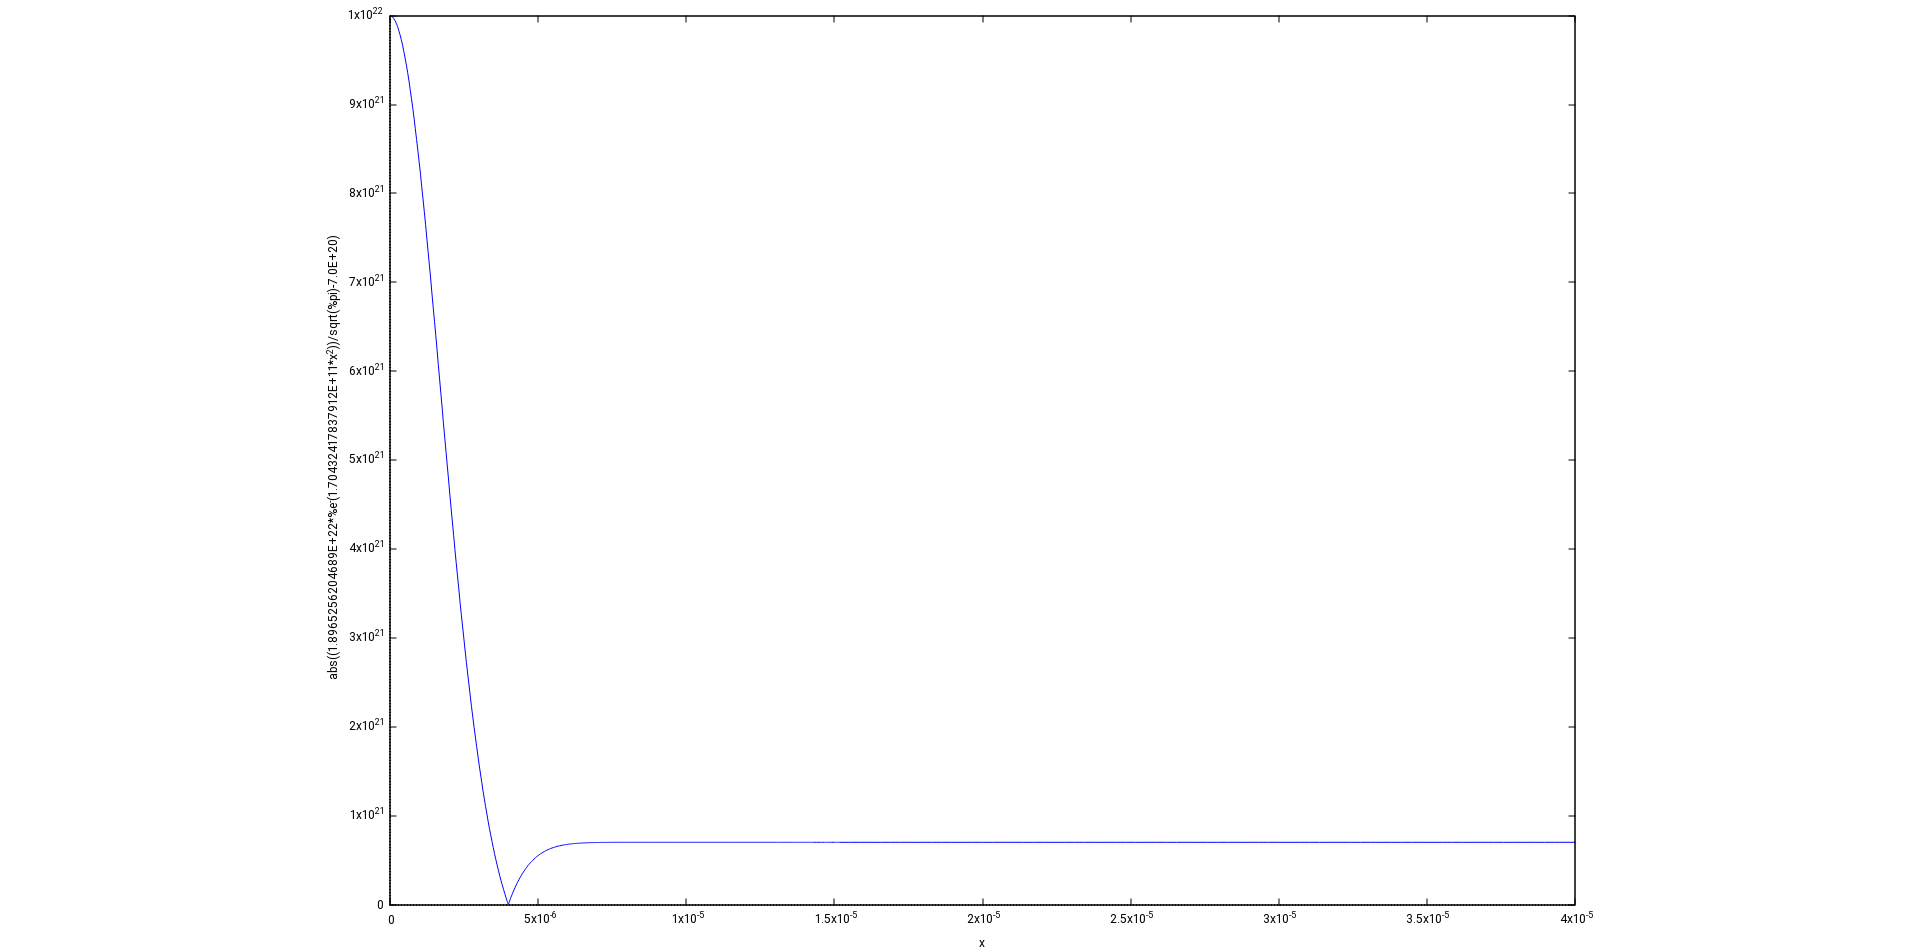
\includegraphics[width=0.75\textwidth]{n-well-diffusion.png}
	\caption{Dopant concentration after 12 hours}
	\label{nwell_drive_in_outcome}
\end{figure}

TODO